% MonSTAR user data handling statement for the Monash Student Association.
% Every claim comes from the source code at the commit named in Section 1.2.
% Re-check the claims and bump that commit whenever the data model changes.
%
% Build:  latexmk -pdf data-handling.tex && latexmk -c
% Before sending, resolve every \todo:  grep -n '\\todo{' data-handling.tex

\documentclass[11pt,a4paper]{article}

% --- Page geometry ------------------------------------------------------------
\usepackage[a4paper,margin=1in]{geometry}

% --- Graphics, colour ---------------------------------------------------------
\usepackage{graphicx}
\usepackage{xcolor}

% --- Tables -------------------------------------------------------------------
\usepackage{booktabs}
\usepackage{tabularx}
\newcolumntype{L}{>{\raggedright\arraybackslash}X}
\newcolumntype{P}[1]{>{\raggedright\arraybackslash}p{#1}}

% --- Headers / footers --------------------------------------------------------
\usepackage{fancyhdr}

% --- Hyperlinks ---------------------------------------------------------------
\usepackage{hyperref}
\hypersetup{pdftitle={MonSTAR user data handling statement},
            pdfauthor={WIRED Monash}}

% --- Header / footer layout ---------------------------------------------------
\pagestyle{fancy}
\fancyhf{}
\fancyhead[L]{\itshape\small\rightmark}
\fancyfoot[C]{\thepage}
\renewcommand{\headrulewidth}{0.4pt}
\renewcommand{\footrulewidth}{0pt}
% Header names the first section on the page (\leftmark would show the last).
\renewcommand{\sectionmark}[1]{\markright{\thesection.\ \MakeUppercase{#1}}}
\renewcommand{\subsectionmark}[1]{}

% --- Shortcuts ----------------------------------------------------------------
% A fact the code cannot show. Fill in from the service dashboards.
\newcommand{\todo}[1]{\textcolor{red}{\textbf{[TODO: #1]}}}

% --------------------------------- Metadata --------------------------------- %
\title{MonSTAR\\User data handling statement}
\author{WIRED Monash}
\date{27 September 2026}

\begin{document}
\hypersetup{pageanchor=false}

% -------------------------------- Title page -------------------------------- %
\begin{titlepage}
  \centering
  \vspace*{5\baselineskip}
  {\huge\bfseries MonSTAR\par}
  {\huge\bfseries User data handling statement\par}
  \vspace{3\baselineskip}
  {\large\bfseries Report for the Monash Student Association\par}
  \vspace{0.3\baselineskip}
  {\small By Jenul Ferdinand \quad WIRED Monash\par}
  \vfill
  {\small Jenul Ferdinand\par}
  \vspace{0.8\baselineskip}
  {\small 27 September 2026\par}
  \vspace*{2\baselineskip}
\end{titlepage}

% ----------------------------- Table of contents ---------------------------- %
\clearpage
\hypersetup{pageanchor=true}
\pagenumbering{roman}
\thispagestyle{plain}
\tableofcontents
\clearpage
\pagenumbering{arabic}

\section{Overview}

% =========================================================================== %
\subsection{About MonSTAR}
% =========================================================================== %

MonSTAR (\href{https://monstar.wired.org.au}{monstar.wired.org.au}) is a unit
review site for Monash University students.  The Projects Team at WIRED
Monash, the student society of the Faculty of Information Technology, builds
and runs it.  Anyone can read unit pages and reviews without an account.
Signed-in users can write reviews, like or dislike other people's reviews,
and get a notification when someone likes theirs.

Only Monash accounts can sign in: student addresses of the form
\nolinkurl{abcd1234@student.monash.edu} and staff addresses of the form
\nolinkurl{first.last@monash.edu}.  Google handles sign-in.  MonSTAR has not
offered password sign-in since February 2025.

% =========================================================================== %
\subsection{About this statement}
% =========================================================================== %

This statement sets out what personal data MonSTAR collects, why it needs it,
where the data lives, who can see it, how we protect it, how long we keep it,
and how users can see, correct or delete it.  We organised it around the
questions that privacy frameworks such as the Australian Privacy Principles
and the GDPR ask of a service.  It describes the system and makes no legal
assessment.  Users can read a shorter version on the site's privacy page,
\href{https://monstar.wired.org.au/privacy}{monstar.wired.org.au/privacy},
which the footer and the sign-in page link to.

We wrote it from MonSTAR's source code, which is public at
\href{https://github.com/wiredmonash/monstar}{\nolinkurl{github.com/wiredmonash/monstar}},
so you can check any claim here against the code.  It reflects commit
\texttt{f70f0af} on the \texttt{main} branch.  A few facts, such as hosting
regions, come from the running services instead.

% =========================================================================== %
\subsection{Summary}
% =========================================================================== %

\begin{itemize}
  \item MonSTAR keeps a small account record: Monash email address, Google
    account ID, username, profile picture and an admin flag.  It does not ask
    for phone numbers, postal addresses, student ID numbers, dates of birth
    or payment details, and it discards the name on the Google account.
  \item Reviews are public.  Each one shows its author's username and profile
    picture, which default to the student's authcate and Google profile
    photo.  Users can change both.
  \item Public pages and API responses show no account data beyond the
    username and profile picture.  Email addresses stay private.
  \item MongoDB Atlas holds the data and Vercel runs the site, both in
    Sydney.  Cloudinary stores uploaded profile pictures in the United
    States (Section~\ref{sec:where}).
  \item Users can delete their account from their profile page.  MonSTAR
    deletes their reviews, notifications, votes and uploaded picture in the
    same step (Section~\ref{sec:retention}).
  \item Section~\ref{sec:gaps} lists the gaps we found while writing this
    statement.
\end{itemize}

\section{What we collect}
\label{sec:collect}

% =========================================================================== %
\subsection{Account data}
% =========================================================================== %

MonSTAR creates an account the first time someone signs in.  Google sends a
signed token that includes the account's email address, account ID, name and
profile photo.  MonSTAR keeps the fields in Table~\ref{tab:account} and
discards the name.

\begin{table}[htbp]
  \centering
  \small
  \renewcommand{\arraystretch}{1.25}
  \begin{tabularx}{\textwidth}{@{}P{2.7cm}LLP{2.5cm}@{}}
    \toprule
    \textbf{Data} & \textbf{Source} & \textbf{Why we keep it}
      & \textbf{Who can see it} \\
    \midrule
    Email address & Google sign-in
      & Limit sign-in to Monash accounts and find the account at each sign-in
      & The user and admins \\
    Google account ID & Google sign-in
      & Link the Google account to the MonSTAR account
      & No one; the API never returns it \\
    Username & The part of a student email before the @ (the authcate), or
      the first name in a staff email
      & Show who wrote a review
      & Public \\
    Profile picture & A link to the Google profile photo, or a picture the
      user uploads
      & Show next to the user's reviews
      & Public \\
    Admin flag & Set by MonSTAR
      & Grant moderation rights
      & The user and admins \\
    Liked and disliked reviews & The user's votes
      & Let each user vote once per review
      & The user and admins \\
    Notifications & Created when someone likes the user's review
      & Tell the user who liked it
      & The user \\
    Session token hash & Created at sign-in
      & Keep the user signed in (Section~\ref{sec:sessions})
      & No one \\
    \bottomrule
  \end{tabularx}
  \caption{Fields in a MonSTAR account.}
  \label{tab:account}
\end{table}

The record also holds housekeeping fields: a flag for Google sign-in and
links to the user's reviews and notifications.  People with access to the
database itself can read every field (Section~\ref{sec:infra}).

Because the default username is the student's authcate, anyone who can search
the Monash directory can find out who wrote a review until the student
changes it.  Users can change their username and upload a different picture
from their profile page.

% =========================================================================== %
\subsection{Reviews, votes and notifications}
% =========================================================================== %

A review holds a title, the review text, the semester and year the student
took the unit, an optional grade (HD, D, C, P or N), four ratings from 0 to
5, like and dislike counts, and the times it was created and last edited.
Reviews are public and show the author's username and profile picture.

Like and dislike counts are public; the list of reviews a user voted on is
private.  Liking a review sends its author a notification with the liker's
username and profile picture, so authors can see who liked their reviews.
Dislikes send no notification.

% =========================================================================== %
\subsection{Analytics, cookies and browser storage}
% =========================================================================== %

MonSTAR uses Vercel Web Analytics to count page views.  It sets no cookies.
For each page view Vercel records the time, the page address, the referring
site, a location derived from the request (country, region and city), and
the device type, operating system and browser.  Profile page addresses reach
Vercel with the username replaced by a placeholder.  Vercel tells visitors apart
with a hash of the request, discards that hash after 24 hours, and shows us
only aggregate figures.\footnote{Vercel, \emph{Privacy and Compliance} (Web
Analytics), \url{https://vercel.com/docs/analytics/privacy-policy}.}

The site sets two cookies, both for sign-in (Section~\ref{sec:sessions}).  It
also keeps display preferences for the unit list, such as sort order and
filters, in the browser's local storage.  MonSTAR does not store those
preferences on its servers.

\section{Where the data lives}
\label{sec:where}

Figure~\ref{fig:containers} shows MonSTAR's parts and the outside services
they talk to.  Table~\ref{tab:services} lists the user data each service
handles.

\begin{figure}[htbp]
  \centering
  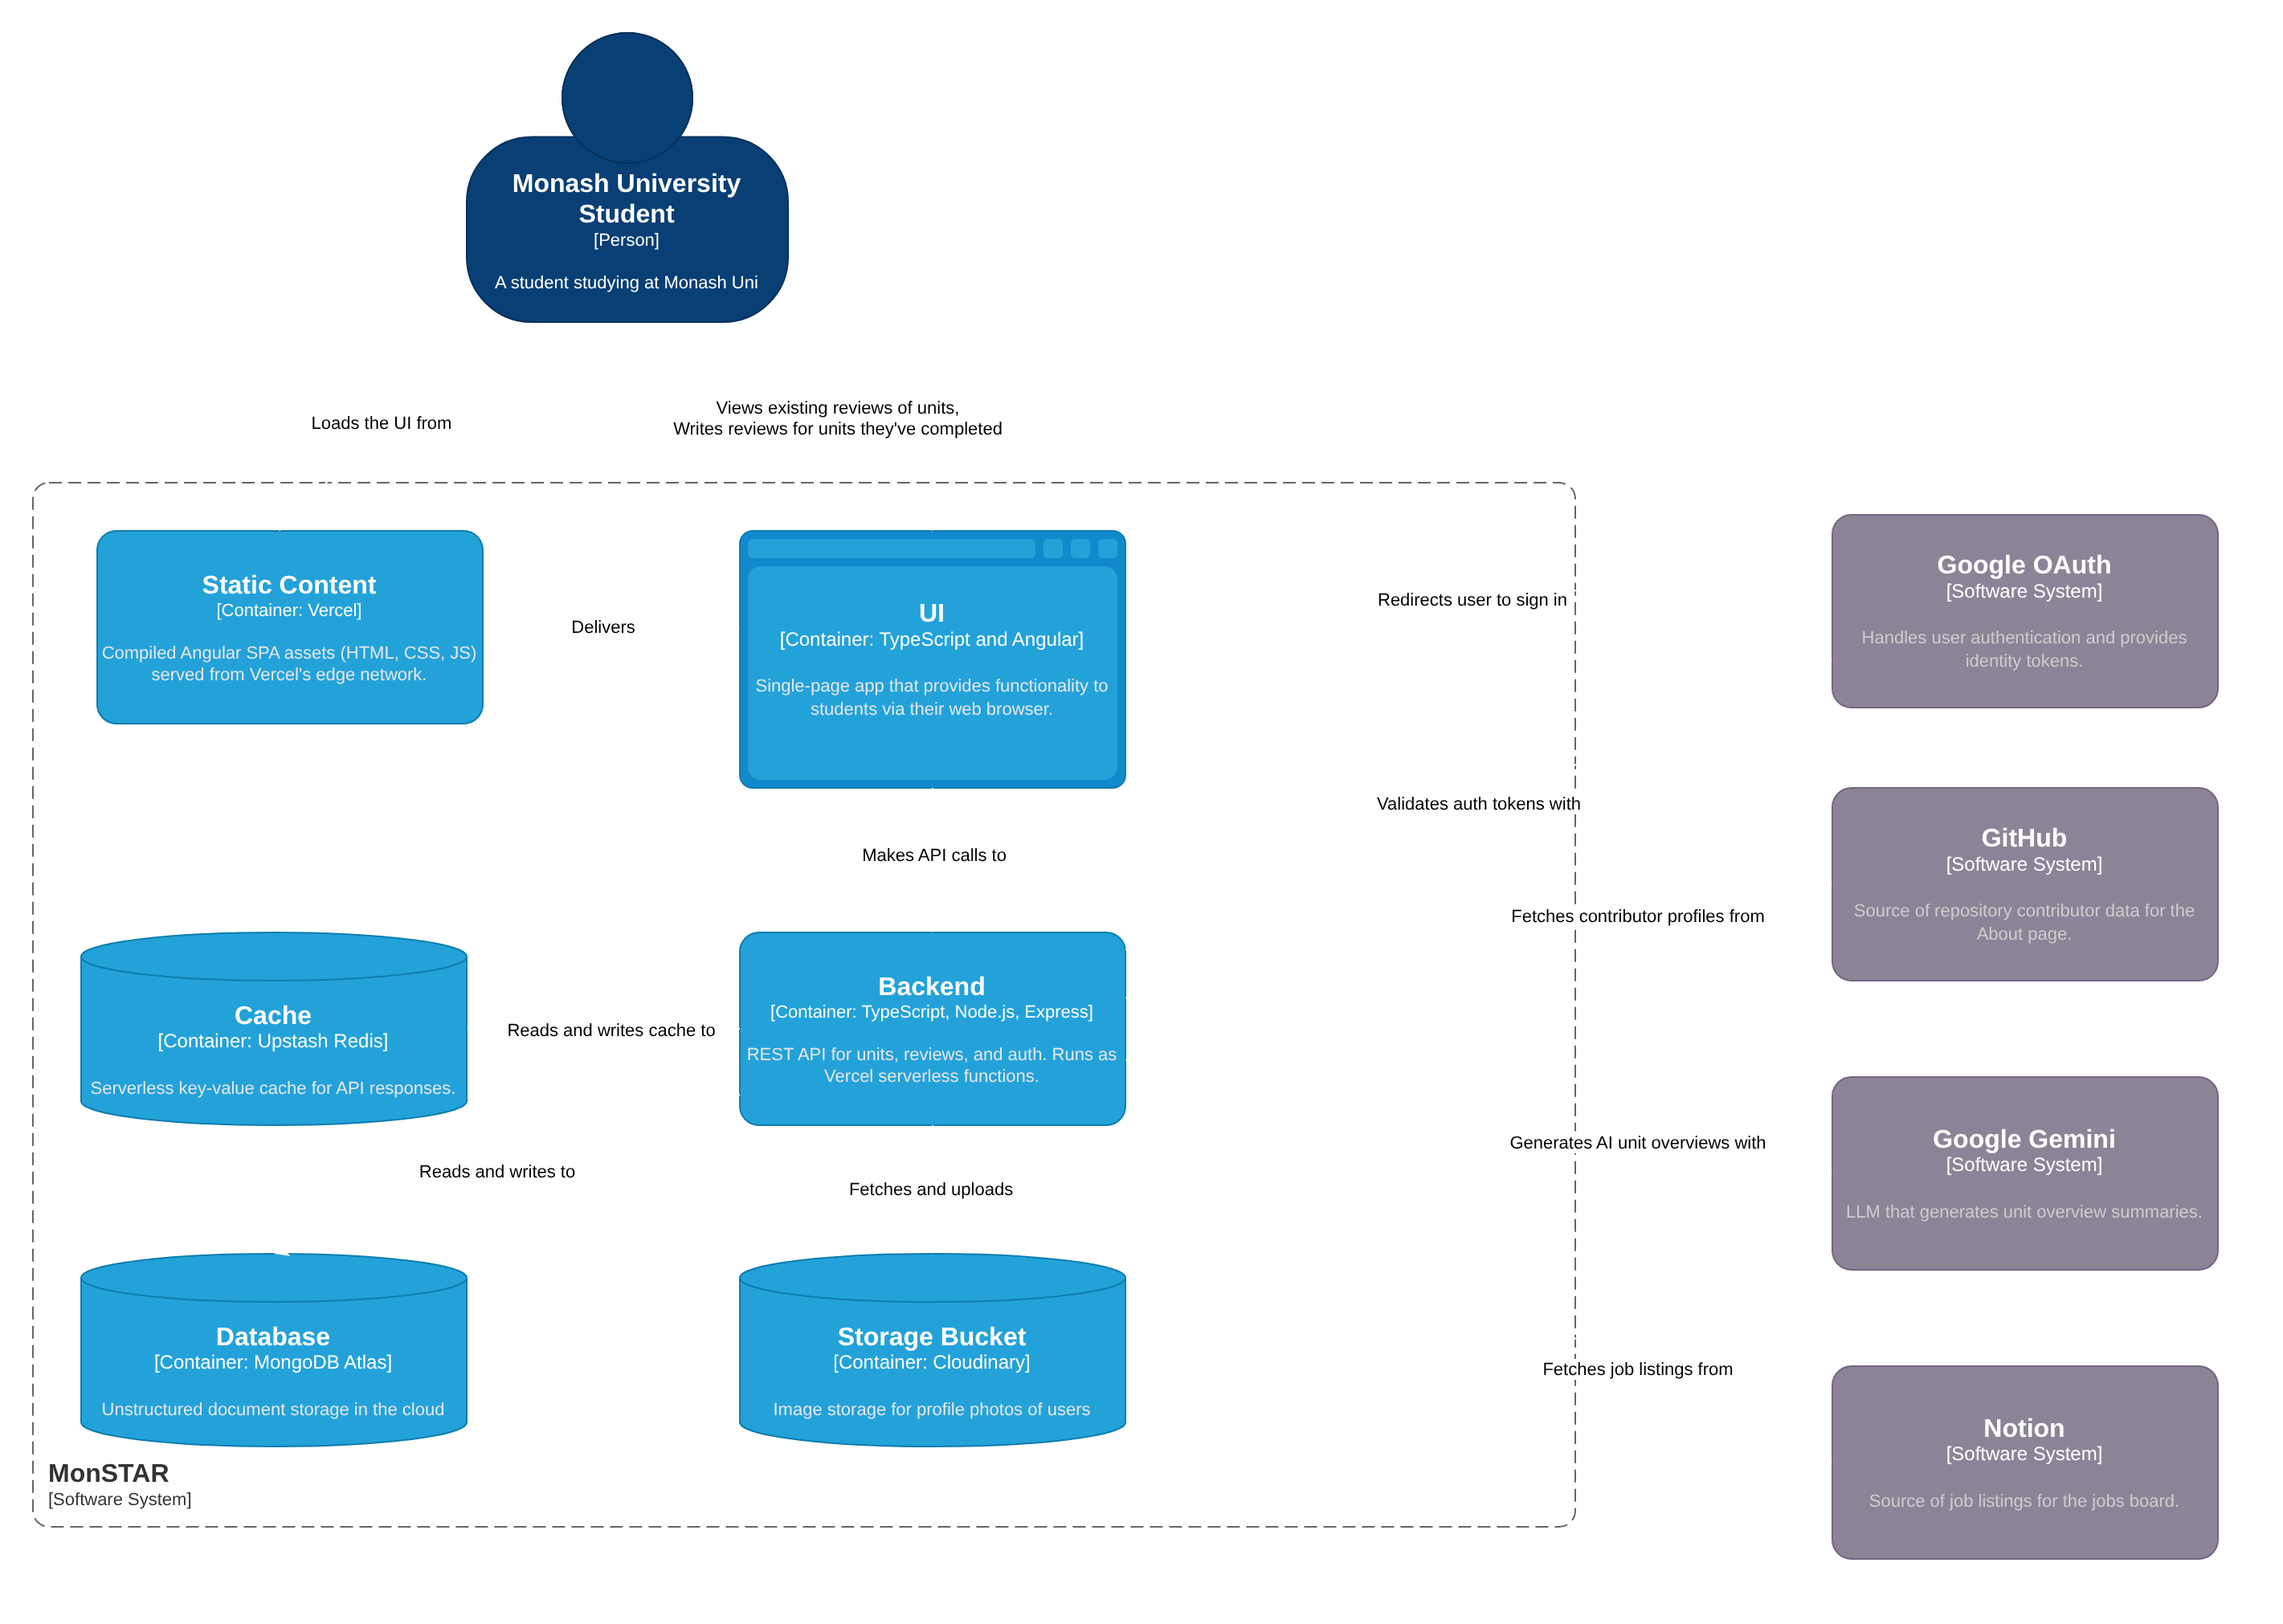
\includegraphics[width=\textwidth]{../2_Container_Diagram.png}
  \caption{MonSTAR's containers and the outside services it uses.}
  \label{fig:containers}
\end{figure}

\begin{table}[htbp]
  \centering
  \small
  \renewcommand{\arraystretch}{1.25}
  \begin{tabularx}{\textwidth}{@{}P{2.4cm}LLP{3cm}@{}}
    \toprule
    \textbf{Service} & \textbf{Role} & \textbf{User data it handles}
      & \textbf{Region} \\
    \midrule
    MongoDB Atlas & Main database
      & Everything in Section~\ref{sec:collect}
      & AWS Sydney (ap-southeast-2) \\
    Vercel & Serves the site, runs the backend API and counts page views
      & All API traffic in transit, server logs, page-view analytics
      & Sydney (syd1) \\
    Cloudinary & Stores uploaded profile pictures
      & Pictures users upload
      & United States (Cloudinary's default) \\
    Google Sign-In & Confirms who is signing in
      & Email address, account ID, name and photo, sent at sign-in
      & Google (global) \\
    Google Gemini API & Writes the AI overview on each unit page
      & Each unit's review titles, text, semesters, years, grades and
        ratings; no usernames, emails or account IDs
      & Google (global) \\
    Upstash Redis & Caches popular units and the jobs board
      & Review titles, text and ratings for the most-reviewed units; no
        author details
      & AWS Sydney (ap-southeast-2) \\
    \bottomrule
  \end{tabularx}
  \caption{Outside services that store or process user data.}
  \label{tab:services}
\end{table}

The AI overview prompt carries no account details, but review text is
whatever the author wrote, so it can mention people.  Nothing calls Gemini
automatically, and the deployed site has no route that can.  A developer
regenerates overviews by hand, running the backend on their own machine
against the production database.  MonSTAR uses the Gemini API's free tier,
where Google's terms let it use prompts to improve its products and allow
human reviewers to read them.\footnote{Google, \emph{Gemini API Additional
Terms of Service}, \url{https://ai.google.dev/gemini-api/terms}.}

Two more services feed MonSTAR but hold no user data.  Notion supplies the
listings on the jobs board, and GitHub supplies the contributor list on the
About page.

% =========================================================================== %
\subsection{Encryption}
% =========================================================================== %

The site redirects plain HTTP to HTTPS and sends a Strict-Transport-Security
header, so browsers use HTTPS on every later visit.  Atlas requires TLS on
every database connection and encrypts its storage and snapshots at rest with
AES-256.\footnote{\raggedright MongoDB, \emph{Configure Security Features for Clusters},
\url{https://www.mongodb.com/docs/atlas/setup-cluster-security/}.}

\section{Who can see the data}
\label{sec:access}

% =========================================================================== %
\subsection{The public}
% =========================================================================== %

Anyone can read reviews, like and dislike counts, and public profiles without
signing in.  A public profile shows a username, a profile picture and that
user's reviews.  The public API returns the same fields.  It never returns
email addresses, Google account IDs, vote lists or session data.

% =========================================================================== %
\subsection{Signed-in users}
% =========================================================================== %

A signed-in user can see their own email address, votes and notifications.
They can change their username and profile picture, edit or delete their own
reviews, and delete their account.  They cannot change anyone else's data.

% =========================================================================== %
\subsection{MonSTAR admins}
% =========================================================================== %

Accounts with the admin flag moderate the site.  One account has it: Jenul
Ferdinand's.  Admins can list every user, including email addresses, change
usernames, and edit or delete any review or account.  The server checks admin
rights on every admin request.

% =========================================================================== %
\subsection{Infrastructure access}
\label{sec:infra}
% =========================================================================== %

Anyone who can log in to MonSTAR's Atlas, Vercel, Cloudinary, Upstash or
Google Cloud accounts can reach the data those services hold
(Table~\ref{tab:infra}).  So can anyone with the production database
connection string, which developers keep on their own machines for tasks such
as regenerating AI overviews.  That string's database user can read and write
every database on the cluster.

Preview deployments, which Vercel builds for each branch except Dependabot's,
use the same database and secrets.  Vercel's login protection limits who can open them, and
builds from forks need our approval.  Anyone who can push a branch to the
repository can still run code against production data.

\begin{table}[htbp]
  \centering
  \small
  \renewcommand{\arraystretch}{1.25}
  \begin{tabularx}{\textwidth}{@{}P{3.6cm}L@{}}
    \toprule
    \textbf{Account} & \textbf{Who has access} \\
    \midrule
    GitHub repository & 5 admins and 9 other accounts can push; 4 can only
      read.  The WIRED Monash organisation requires two-factor
      authentication. \\
    Vercel & The club's shared account (owner), which signs in with a
      passkey, and one team member.  Both use two-factor authentication. \\
    Upstash & Managed through Vercel's storage integration. \\
    MongoDB Atlas & Two organisation owners, one project owner, and one
      account that can build MongoDB Charts from the data.  The organisation
      does not require multi-factor authentication. \\
    Cloudinary & Only Jenul Ferdinand. \\
    Google Cloud (sign-in client and Gemini key) & Only Jenul Ferdinand. \\
    \bottomrule
  \end{tabularx}
  \caption{Who can log in to the services that hold user data.}
  \label{tab:infra}
\end{table}

\section{How we protect it}
\label{sec:security}

% =========================================================================== %
\subsection{Sign-in}
% =========================================================================== %

\begin{itemize}
  \item Google handles authentication.  The backend checks each Google
    token's signature and confirms Google issued it for MonSTAR before
    trusting it.
  \item The backend then checks the email address against the Monash student
    and staff formats and rejects any other address.
  \item MonSTAR has no password sign-in, and no account in the database
    holds a password.
\end{itemize}

% =========================================================================== %
\subsection{Sessions}
\label{sec:sessions}
% =========================================================================== %

After sign-in the backend sets two cookies:
\begin{itemize}
  \item \texttt{access\_token}, a signed token that identifies the user on
    each request and expires after 15 minutes;
  \item \texttt{refresh\_token}, a random 40-byte value that lasts 180 days
    and lets the browser get a new access token without signing in again.
\end{itemize}
The database stores only a SHA-256 hash of the refresh token, so someone
holding a copy of the database still cannot sign in as a user.  Each refresh
swaps the refresh token for a new one, and signing out deletes the stored
hash.  Both cookies are Secure, so browsers send them only over HTTPS, and
HttpOnly, so page scripts cannot read them.  They are also SameSite=Strict, so
browsers do not send them with requests that start on other sites.

% =========================================================================== %
\subsection{Permissions and secrets}
% =========================================================================== %

\begin{itemize}
  \item The server lets only a review's author or an admin edit or delete
    it, and only the account owner or an admin change a username or delete
    an account.
  \item API keys and the token-signing secret live in Vercel's environment
    settings.  The public repository holds only a template with placeholder
    values.
  \item Atlas accepts database connections from any network address,
    because Vercel's functions have no fixed addresses on our plan.  The
    database password is the barrier.
\end{itemize}

% =========================================================================== %
\subsection{Responding to a breach}
% =========================================================================== %

Whoever suspects a breach tells Jenul Ferdinand straight away.  We contain it
first, by rotating the exposed secrets and cutting off access, then work out
what data was exposed.  We tell MSA within 72 hours of confirming a breach,
and email affected users as soon as we know who they are.

\section{How long we keep it}
\label{sec:retention}

% =========================================================================== %
\subsection{Retention}
% =========================================================================== %

MonSTAR keeps account data, reviews, votes and notifications until the user
deletes them or their account.  Only sessions expire on their own: access
tokens after 15 minutes and refresh tokens after 180 days.

Some copies outlast the original:
\begin{itemize}
  \item The popular-units cache in Upstash holds review text and ratings,
    without author details, for up to one week.
  \item Each unit's AI overview summarises the reviews the unit had when a
    developer last regenerated it.  A deleted review still shapes that summary
    until the next regeneration.
  \item The backend logs internal user IDs, not names or emails, when it
    deletes an account.  Vercel keeps runtime logs for one hour on our
    plan.\footnote{Vercel, \emph{Runtime Logs},
    \url{https://vercel.com/docs/logs/runtime}.}
\end{itemize}
The database has no backups.  It runs on Atlas's free tier, which does not
take them, so deleted data leaves no copy behind, and data lost by mistake
cannot be restored (Section~\ref{sec:gaps}).

% =========================================================================== %
\subsection{Deleting an account}
% =========================================================================== %

Users delete their account with the \emph{Delete account} button on their
profile page, then confirm.  MonSTAR then:
\begin{enumerate}
  \item deletes all of the user's reviews and recalculates the average
    ratings of the units they reviewed;
  \item deletes the notifications addressed to the user;
  \item removes the user's likes and dislikes from other people's reviews;
  \item deletes the user's uploaded profile picture from Cloudinary, if they
    uploaded one;
  \item deletes the account record.
\end{enumerate}
Steps 1 to 3 run in one database transaction, so if any of them fails,
MonSTAR deletes nothing and keeps the account.  Notifications the user caused
by liking other people's reviews survive the deletion.  They stay in those
people's inboxes, with the user's username and picture link
(Section~\ref{sec:gaps}).

\section{Users' control over their data}
\label{sec:rights}

Table~\ref{tab:rights} shows how users see, correct and delete their data.

\begin{table}[htbp]
  \centering
  \small
  \renewcommand{\arraystretch}{1.25}
  \begin{tabularx}{\textwidth}{@{}P{3.4cm}L@{}}
    \toprule
    \textbf{Request} & \textbf{How users do it} \\
    \midrule
    See their data & Signed-in users see their profile, reviews and
      notifications on the site.  For a full copy, they email
      \href{mailto:monstarapp@gmail.com}{monstarapp@gmail.com} from their
      Monash address, and we reply within 30 days with their account record,
      reviews and notifications. \\
    Correct it & Change their username and picture on the profile page, and
      edit their reviews at any time. \\
    Delete it & Delete single reviews, or the whole account
      (Section~\ref{sec:retention}). \\
    Ask a question or complain & Email
      \href{mailto:monstarapp@gmail.com}{monstarapp@gmail.com}, the contact
      on the site's terms page. \\
    \bottomrule
  \end{tabularx}
  \caption{How users exercise control over their data.}
  \label{tab:rights}
\end{table}

\section{Known gaps}
\label{sec:gaps}

We found these while preparing this statement.

\begin{enumerate}
  \item \textbf{Identifying default usernames.}  New student accounts take
    the authcate as their public username and the Google profile photo as
    their picture (Section~\ref{sec:collect}).  In September 2026, 553 of
    646 student accounts still used their authcate.
  \item \textbf{Production secrets reach beyond production.}  Developers
    keep the production database connection string locally, and its database
    user can read and write every database on the shared cluster.  Vercel
    also gives every branch preview the production database connection
    string and token-signing secret, so all 14 accounts that can push to
    GitHub can reach production data.  Dependabot's branches no longer build
    previews, so its dependency updates reach these secrets only after
    someone reviews and merges them.  Issue \#331 covers a least-privilege
    database user.  Previews also need their own database and secrets, and the
    GitHub, Vercel and Atlas access lists need a review.
  \item \textbf{No database backups.}  The free Atlas tier takes none, so an
    accidental deletion or a bad write cannot be undone.  A scheduled export
    or a paid tier would fix this.
  \item \textbf{Notifications outlive the liker's account.}  Deleting an
    account leaves its ``liked your review'' notifications in other users'
    inboxes (Section~\ref{sec:retention}).
  \item \textbf{Gemini free tier.}  Google may use review text sent for AI
    overviews to improve its products (Section~\ref{sec:where}).
  \item \textbf{No rate limits on public endpoints.}  Someone could download
    every public review with its author's username.  Issues \#328 and \#329
    in our repository track the fix.
\end{enumerate}

\end{document}
